%==========================================
%
% Sibgrapi 2015 paper
%
%==========================================


% Note that the a4paper option is mainly intended so that authors in
% countries using A4 can easily print to A4 and see how their papers will
% look in print - the typesetting of the document will not typically be
% affected with changes in paper size (but the bottom and side margins will).
% Use the testflow package mentioned above to verify correct handling of
% both paper sizes by the user's LaTeX system.
%
% Also note that the "draftcls" or "draftclsnofoot", not "draft", option
% should be used if it is desired that the figures are to be displayed in
% draft mode.
%
\documentclass[10pt, conference]{IEEEtran}

% *** MISC UTILITY PACKAGES ***
%
%\usepackage{ifpdf}
% Heiko Oberdiek's ifpdf.sty is very useful if you need conditional
% compilation based on whether the output is pdf or dvi.
% usage:
% \ifpdf
%   % pdf code
% \else
%   % dvi code
% \fi
% The latest version of ifpdf.sty can be obtained from:
% http://www.ctan.org/tex-archive/macros/latex/contrib/oberdiek/
% Also, note that IEEEtran.cls V1.7 and later provides a builtin
% \ifCLASSINFOpdf conditional that works the same way.
% When switching from latex to pdflatex and vice-versa, the compiler may
% have to be run twice to clear warning/error messages.






% *** CITATION PACKAGES ***
%
%\usepackage{cite}
% cite.sty was written by Donald Arseneau
% V1.6 and later of IEEEtran pre-defines the format of the cite.sty package
% \cite{} output to follow that of IEEE. Loading the cite package will
% result in citation numbers being automatically sorted and properly
% "compressed/ranged". e.g., [1], [9], [2], [7], [5], [6] without using
% cite.sty will become [1], [2], [5]--[7], [9] using cite.sty. cite.sty's
% \cite will automatically add leading space, if needed. Use cite.sty's
% noadjust option (cite.sty V3.8 and later) if you want to turn this off.
% cite.sty is already installed on most LaTeX systems. Be sure and use
% version 4.0 (2003-05-27) and later if using hyperref.sty. cite.sty does
% not currently provide for hyperlinked citations.
% The latest version can be obtained at:
% http://www.ctan.org/tex-archive/macros/latex/contrib/cite/
% The documentation is contained in the cite.sty file itself.






% *** GRAPHICS RELATED PACKAGES ***
%
\usepackage{subimages}
\setfigdir{figs}




% *** MATH PACKAGES ***
%
\usepackage[cmex10]{amsmath}
% A popular package from the American Mathematical Society that provides
% many useful and powerful commands for dealing with mathematics. If using
% it, be sure to load this package with the cmex10 option to ensure that
% only type 1 fonts will utilized at all point sizes. Without this option,
% it is possible that some math symbols, particularly those within
% footnotes, will be rendered in bitmap form which will result in a
% document that can not be IEEE Xplore compliant!
%
% Also, note that the amsmath package sets \interdisplaylinepenalty to 10000
% thus preventing page breaks from occurring within multiline equations. Use:
\interdisplaylinepenalty=2500
% after loading amsmath to restore such page breaks as IEEEtran.cls normally
% does. amsmath.sty is already installed on most LaTeX systems. The latest
% version and documentation can be obtained at:
% http://www.ctan.org/tex-archive/macros/latex/required/amslatex/math/
\usepackage{amsthm}
\newtheorem{definition}{Definition}





% *** SPECIALIZED LIST PACKAGES ***
%
%\usepackage{algorithmic}
% algorithmic.sty was written by Peter Williams and Rogerio Brito.
% This package provides an algorithmic environment fo describing algorithms.
% You can use the algorithmic environment in-text or within a figure
% environment to provide for a floating algorithm. Do NOT use the algorithm
% floating environment provided by algorithm.sty (by the same authors) or
% algorithm2e.sty (by Christophe Fiorio) as IEEE does not use dedicated
% algorithm float types and packages that provide these will not provide
% correct IEEE style captions. The latest version and documentation of
% algorithmic.sty can be obtained at:
% http://www.ctan.org/tex-archive/macros/latex/contrib/algorithms/
% There is also a support site at:
% http://algorithms.berlios.de/index.html
% Also of interest may be the (relatively newer and more customizable)
% algorithmicx.sty package by Szasz Janos:
% http://www.ctan.org/tex-archive/macros/latex/contrib/algorithmicx/




% *** ALIGNMENT PACKAGES ***
%
%\usepackage{array}
% Frank Mittelbach's and David Carlisle's array.sty patches and improves
% the standard LaTeX2e array and tabular environments to provide better
% appearance and additional user controls. As the default LaTeX2e table
% generation code is lacking to the point of almost being broken with
% respect to the quality of the end results, all users are strongly
% advised to use an enhanced (at the very least that provided by array.sty)
% set of table tools. array.sty is already installed on most systems. The
% latest version and documentation can be obtained at:
% http://www.ctan.org/tex-archive/macros/latex/required/tools/


%\usepackage{mdwmath}
%\usepackage{mdwtab}
% Also highly recommended is Mark Wooding's extremely powerful MDW tools,
% especially mdwmath.sty and mdwtab.sty which are used to format equations
% and tables, respectively. The MDWtools set is already installed on most
% LaTeX systems. The lastest version and documentation is available at:
% http://www.ctan.org/tex-archive/macros/latex/contrib/mdwtools/


% IEEEtran contains the IEEEeqnarray family of commands that can be used to
% generate multiline equations as well as matrices, tables, etc., of high
% quality.


%\usepackage{eqparbox}
% Also of notable interest is Scott Pakin's eqparbox package for creating
% (automatically sized) equal width boxes - aka "natural width parboxes".
% Available at:
% http://www.ctan.org/tex-archive/macros/latex/contrib/eqparbox/



% *** PDF, URL AND HYPERLINK PACKAGES ***
%
\usepackage{hyperref}





% *** Do not adjust lengths that control margins, column widths, etc. ***
% *** Do not use packages that alter fonts (such as pslatex).         ***
% There should be no need to do such things with IEEEtran.cls V1.6 and later.
% (Unless specifically asked to do so by the journal or conference you plan
% to submit to, of course. )


% correct bad hyphenation here
\hyphenation{op-tical net-works semi-conduc-tor}


\begin{document}
%
% paper title
% can use linebreaks \\ within to get better formatting as desired
\title{Visualization tool for comparison of a single amino acid change in protein simulation}

%------------------------------------------------------------------------- 
% change the % on next lines to produce the final camera-ready version 
\newif\iffinal
%\finalfalse
\finaltrue
\newcommand{\jemsid}{99999}
%------------------------------------------------------------------------- 

% author names and affiliations
% use a multiple column layout for up to two different
% affiliations

\iffinal
  \author{%
    \IEEEauthorblockN{Bruno Iochins Grisci}
    \IEEEauthorblockA{%
      Instituto de Informatica\\
      UFRGS\\
      Porto Alegre, Brazil\\
      Email:  \href{mailto:bigrisci@inf.ufrgs.br}{bigrisci@inf.ufrgs.br}}
  }
\else
  \author{Sibgrapi paper ID: \jemsid \\ }
\fi

% for over three affiliations, or if they all won't fit within the width
% of the page, use this alternative format:
% 
%\author{\IEEEauthorblockN{Michael Shell\IEEEauthorrefmark{1},
%Homer Simpson\IEEEauthorrefmark{2},
%James Kirk\IEEEauthorrefmark{3}, 
%Montgomery Scott\IEEEauthorrefmark{3} and
%Eldon Tyrell\IEEEauthorrefmark{4}}
%\IEEEauthorblockA{\IEEEauthorrefmark{1}School of Electrical and Computer Engineering\\
%Georgia Institute of Technology,
%Atlanta, Georgia 30332--0250\\ Email: see http://www.michaelshell.org/contact.html}
%\IEEEauthorblockA{\IEEEauthorrefmark{2}Twentieth Century Fox, Springfield, USA\\
%Email: homer@thesimpsons.com}
%\IEEEauthorblockA{\IEEEauthorrefmark{3}Starfleet Academy, San Francisco, California 96678-2391\\
%Telephone: (800) 555--1212, Fax: (888) 555--1212}
%\IEEEauthorblockA{\IEEEauthorrefmark{4}Tyrell Inc., 123 Replicant Street, Los Angeles, California 90210--4321}}


%------------------------------------------------------------------------- 
% Special Sibgrapi teaser
\teaser{%
  \oneimage{Image of the tool with all elements presented.}{.99}{all.png}
}
%------------------------------------------------------------------------- 

% make the title area
\maketitle


\begin{abstract}

% DO NOT USE SPECIAL CHARACTERS, SYMBOLS, OR MATH IN YOUR TITLE OR ABSTRACT.
%
\end{abstract}

\begin{IEEEkeywords}
molecular dynamics simulation; bioinformatics; proteins; protein folding; amino acid mutation; temporal visualization; multidimensional visualization; parallel coordinates; radar chart;

\end{IEEEkeywords}


\IEEEpeerreviewmaketitle


% Wherever Times is specified, Times Roman or Times New Roman may be used. If neither is available on your system, please use the font closest in appearance to Times. Avoid using bit-mapped fonts if possible. True-Type 1 or Open Type fonts are preferred. Please embed symbol fonts, as well, for math, etc.

%==========================================
%==========================================
 %1) Introdução (motivação para o trabalho, objetivos e resultados esperados), 2) Caracterização dos dados e problema/questões que a visualização pretende responder, 3) Descrição da técnica de visualização desenvolvida (incluir aqui informação sobre a implementação, biblioteca ou ferramenta utilizada), 4) Resultados (exemplos de uso), 5) Conclusões. Não há limite de páginas, mas o razoável é de 8 a 12 páginas no máximo.

%==========================================
\section{Introduction}
%

In a molecular dynamics simulation, many features can be measured, depending on the researcher’s interests. One of the mainstays of simulation analysis is the inspection of trajectory convergence, an indication of simulation stability~\cite{grossfield2007convergence}. It is, however, well known that convergence is a subjective matter, and that the evaluation of single structural features (such as RMSD) for this purpose is very unreliable~\cite{knapp2011intuitive}~\cite{van2006biomolecular}. Thus, the simultaneous evaluation of multiple structural analysis via a simple visual tool, as the one presented here, is of great utility to the field of macromolecular simulation.

Proteins are polymers formed by a sequence of around 20 different possible amino acids (Fig.~\ref{fig:aminoacids}) that under physiological conditions fold into a precise shape known as its native state~\cite{anfinsen:1973}. Each amino acid has an alpha carbon (\texttt{CA}) with bonds to amino (\texttt{NH2}) and carboxyl (\texttt{COOH}) groups and a variable side-chain (\texttt{R}) that determines the particular physicochemical properties of each residue. 

\begin{figure}
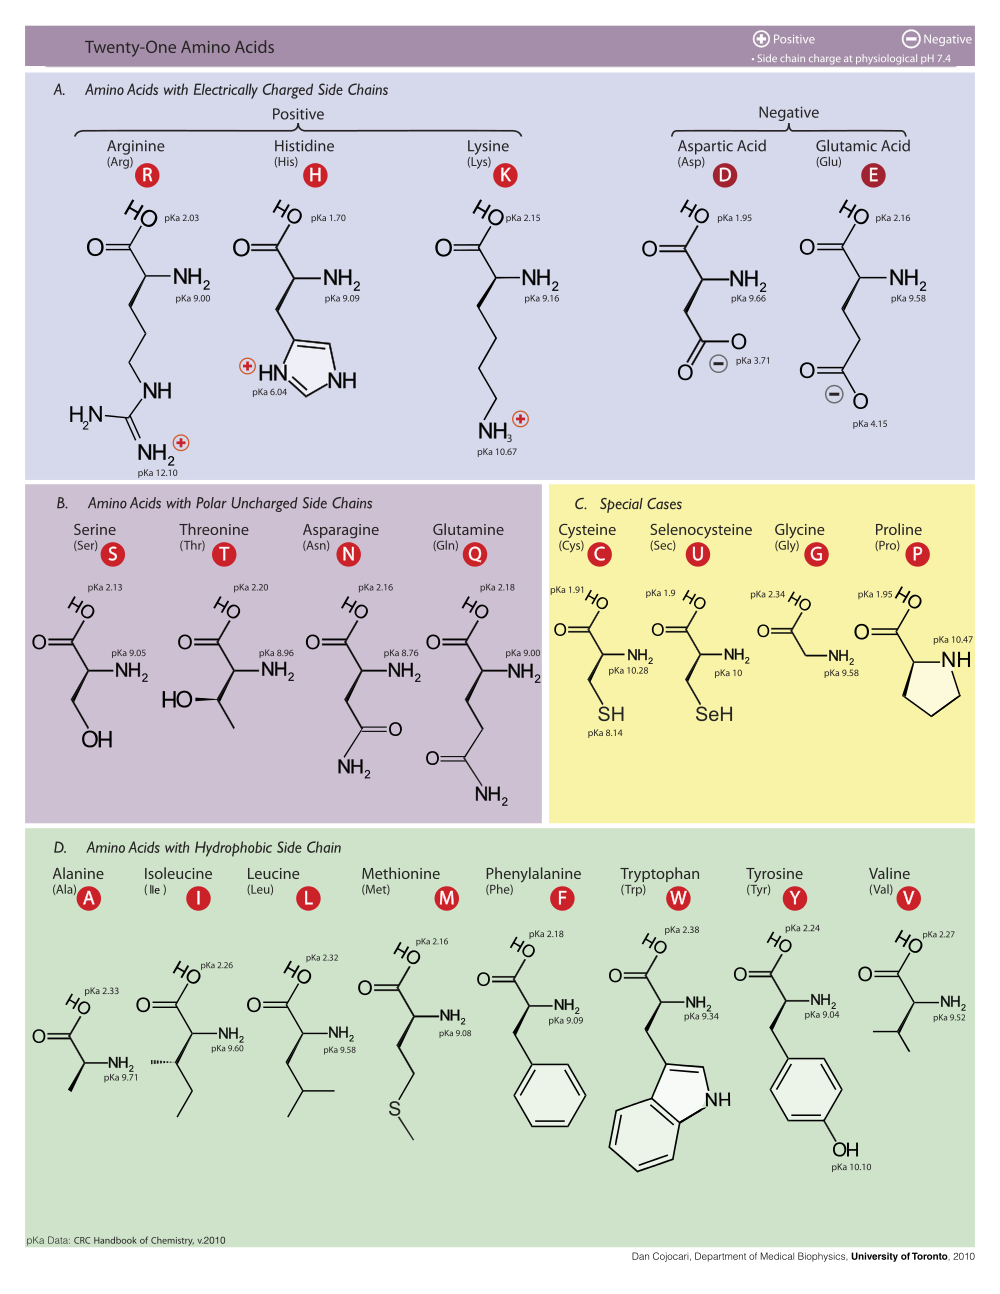
\includegraphics[width=0.8\linewidth]{figs/Amino_Acids.png}
\caption{Table of amino acids physicochemical properties.} 
\label{fig:aminoacids}
\end{figure}

A peptide is a molecule composed of two or more amino acids chained by a chemical bond called the \textit{peptide bond}. This bond is formed when the carboxyl group of one residue reacts with the amino group of the other residue, releasing a water molecule. The interaction between amino acids in a protein causes the polypeptide chain to fold, usually in a proper configuration, as \texttt{$\alpha$-helix}, \texttt{$\beta$-sheet}, \texttt{coil} or \texttt{turn}. These local folding patterns represent the secondary structure of a protein. The topology or fold is given by the succession of secondary structures connected in a \texttt{3D} space. The specific characteristics of the peptide bond have significant implications for the \texttt{3D} fold that can be adopted by polypeptides. The peptide bond (\texttt{C-N}) has a double bond, and it is not allowed rotation of the molecule around this bond. The rotation is only permitted around the bonds \texttt{N-C$\alpha$} and \texttt{C}$_{\alpha}$\texttt{-C}. 

The analysis of experimental protein structures (\texttt{X}-ray data) reveals that amino acid residues can assume many conformations in proteins~\cite{Borguesan:2015}. Each amino acid has a set of physiochemical properties which contributes to its intrinsic conformational preference~\cite{Mathura:2005}. Amino acids in a secondary structure usually adopt a particular set of backbone torsion angles~\cite{Borguesan:2015}.

The amino acids sequence of a protein is directly related to its structure in three dimensional space, which is defining of the protein biological function. The change of only one amino acid in the chain is capable of great modification of the structure and function of a protein because of the differences in size and physical-chemical properties among amino acids~\cite{nelson2008lehninger}.

\subsection{Related work}
%


%==========================================
\section{Data characterization}

The data for testing this visualization tool comes from the Kappa-conotoxin PVIIA, with amino acids sequence: $CRIPNQKCFQHLDDCCSRKCNRFNKCV$. Its three dimensional structure, obtained with nuclear magnetic resonance (NMR) from the Protein Data Bank (PDB) under the code 1AV3, can be seen in Fig.~\ref{fig:pviia}. Kappa-conotoxins are neurotoxical proteins extracted from sea slugs poison. They are inhibitors of the potassium channel and when injected in different organisms some alterations in their effect can be observed, from hyperactivity in fish to death when combined with other variants of conotoxins. The substitution of the asparagine ($N$) in the fifth position in the amino acids chain of the Kappa-conotoxin PVIIA by an alanine ($A$) is know to cause a reduction of 100\% in the toxicity of this protein~\cite{jacobsen2000single}~\cite{mir2016conotoxins}~\cite{akey2002inherited}.

\begin{figure}
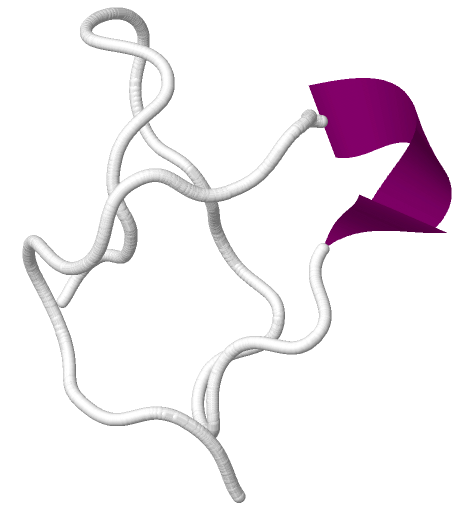
\includegraphics[width=0.7\linewidth]{figs/pviia.png}
\caption{Three dimensional structure of the Kappa-conotoxin PVIIA.} 
\label{fig:pviia}
\end{figure}

For this study, this asparagine was changed by all possible 20 amino acids, and for each resulting structure a molecular dynamics simulation was performed in order to evaluate its behavior during a predetermined period of time under chosen conditions. The simulations were performed with GROMACS~\cite{hess2008gromacs}, a software for biomolecules simulation, with the simulated time of 50ns. These simulations mimic the behavior of biomolecules in a solvent under controled temperature. From the data created versus time, the following attributes were studied.

\subsection{Data dimensions}

\paragraph*{DSSP} Analysis of the secondary structure of the protein for each frame of the simulation. The secondary structure is a local structural conformation of a region in the amino acids sequence which follows specific patterns that, once folded, will originate the three dimensional functional structure of the protein~\cite{kabsch1983dictionary}. 
%

\paragraph*{SASA} Solvent-accessible surface area is the surface area of the protein that is accessible to the solvent. By analysing the area exposed to the solvent, i.e., what is around the protein, it is possible to infer how denatured is the protein, so the greater the SASA value, the greater the denaturation~\cite{richmond1984solvent}.
%

\paragraph*{GYRATE} The radius of gyration can be used as a measurement of the compactness of a protein structure. It describes the overall spread of the molecule and is calculated taking the root mean square distance of the atoms from their common centre of gravity. Greater values of radius of gyration means a less compact protein~\cite{lobanov2008radius}.
%

\paragraph*{ENERGY} This attribute measures the total energy of the system. The energy is a stability indicator, usually comparable, in which systems with less energy will be more stable (less entropy)~\cite{van1998gromos}.
%

\paragraph*{RMSF} The root mean square fluctuation of atomic positions is the measure of the average distance between the atoms of the simulated protein and a well-defined average position~\cite{maiorov1994significance}. 
%

All the dimensions are continuous numerical values. As can be seen, the data of a single simulation is multidimensional and changes over the simulated time.

%==========================================
\section{Technical background}
%

\subsection{Grid}

\subsection{Parallel Coordinates}

\subsection{Radar Chart}

%------------------------------------------------------------------------- 
\section{Technique overview}
%

The proposed visualization technique takes advantage of the use of three different visualization tools working in synchrony, and the capability of changing the data over time. The parallel coordinates and radar chart data is normalized in the range of minimum and maximum values for each dimension along all time steps.

\subsection{Grid}

The grid is an interactive table where the raw values of the data are displayed as in Fig.~\ref{fig:grid}. Its function is to provide a place where the data can be observed with more detail for scientific purposes.

\begin{figure}
\includegraphics[width=0.9\linewidth]{figs/grid.png}
\caption{Overview of the used grid.} 
\label{fig:grid}
\end{figure}
\paragraph*{Item highlighting} When hoving the mouse over a line in the grid, that line is highlited. This operation also reflects on the other charts.
\paragraph*{Item selection} When right-clicking on a line of the grid with the mouse that line is selected and the item is fixed on the charts. The selected line is becomes darker on the parallel coordinates chart.

\subsection{Parallel Coordinates}

The parallel coordinates chart is used to show a global view of the data, displaying all the items in a given time at once and allowing the user to view the general "shape" of the simulations and spread of the values between items.

\begin{figure}
\includegraphics[width=1.0\linewidth]{figs/brush.png}
\caption{Example of use of the brush.} 
\label{fig:brush}
\end{figure}
\paragraph*{Axis brushing} The brush is the filtering operation of the parallel coordinates and can be seen in Fig.~\ref{fig:brush}. Draging the mouse along an axis select the items in that range. This change is reflected on the grid.
\paragraph*{Axis sorting} When double clicking an axis the order of its values is inverted. This change is reflected on the radar chart.
\paragraph*{Axis reordering} When right-clicking an axis and draging it to left or right the axes are reordered. This change is reflected on the radar chart.
\paragraph*{Recoloring by axis selection} The color of the lines of the parallel coordinates is defined by the range of the selected axis. Clicking an axis change the dimension used for coloring. Figures~\ref{fig:dssp} and~\ref{fig:gyrate} show the colors for two different dimensions. This function is useful when analysing one dimension while wanting to keep in mind the behavior of another.

\begin{figure}
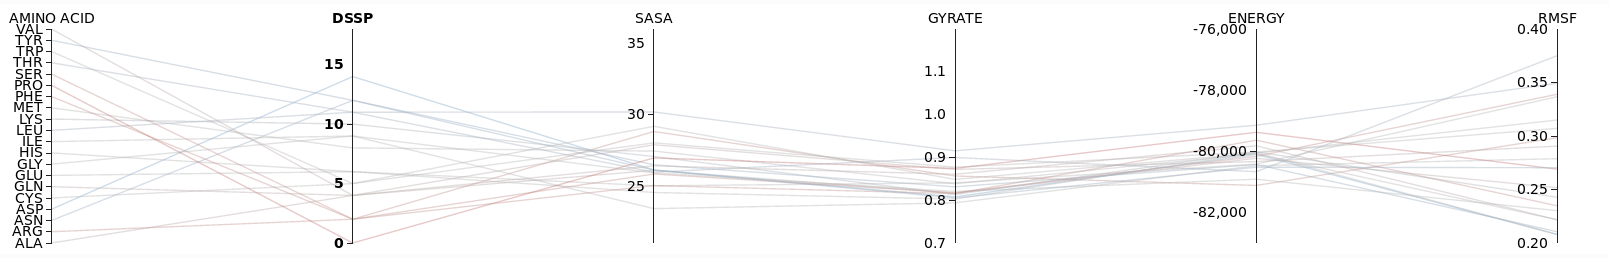
\includegraphics[width=1.0\linewidth]{figs/dssp.png}
\caption{Colors of the parallel coordinates for the DSSP dimension.} 
\label{fig:dssp}
\end{figure}

\begin{figure}
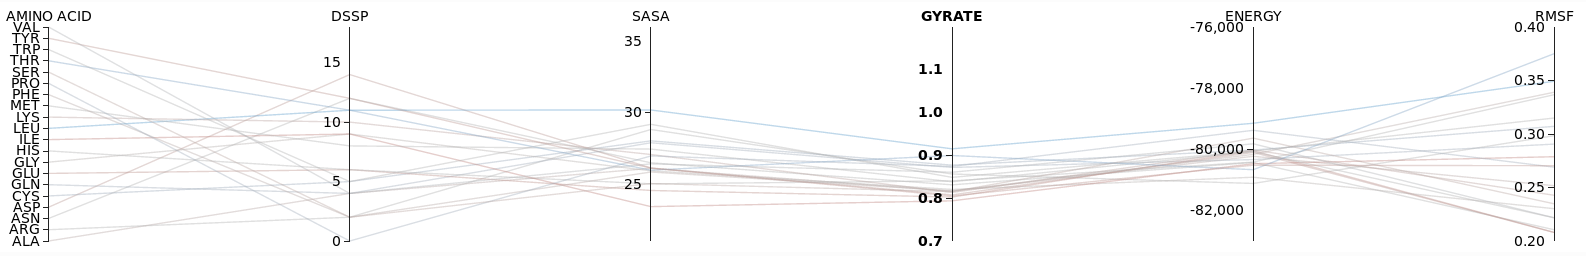
\includegraphics[width=1.0\linewidth]{figs/gyrate.png}
\caption{Colors of the parallel coordinates for the GYRATE dimension.} 
\label{fig:gyrate}
\end{figure}

\subsection{Radar Chart}

The objective of the radar chart, showed in Fig.~\ref{fig:radar}, is to visualize and compare specif items of the data, i.e., single simulations. The hypothesis is that overlaping the shapes of the lines from the parallel coordinates in a radial way makes it easier com see the similarities and differences between a small number of items, while the global view is better represented by the parallel coordinates chart since for many shapes the radar chart becomes convoluted.  

\begin{figure}
\includegraphics[width=0.8\linewidth]{figs/radar.png}
\caption{Example of one simulation being visualized in the radar chart.} 
\label{fig:radar}
\end{figure}
\paragraph*{Item highlighting} When hoving the mouse over a shape in the radar chart or its label, the shape is filled in order to be higlighted.

\subsection{Slider}

The slider is the element that allows the user to change the data being visualized over time (Fig~\ref{fig:slider}). It can be clicked or dragged, then selecting a specific time step of the simulation, and the charts and grid will be updated. It is also possible to visualize the changes in time with animations. For this there are two buttons, "Play" and "Rec", that update the data automatically untill the end of the time steps. Interacting with any other element of the visualization pauses the animation. A text box informs the current time step.

\begin{figure}

\includegraphics[width=0.8\linewidth]{figs/slider.png}
\caption{View of the elements of the slider, that enables the change of time steps.} 
\label{fig:slider}
\end{figure}

%==========================================
\section{Experiments and Discussion}
%

All elements of this visualization tool were implemented using JavaScript, HTML and CSS, with the visualization library D3.js. The parallel coordinates chart uses the visual toolkit for multidimensional detectives Parallel Coordinates (0.7.0) (\url{http://syntagmatic.github.io/parallel-coordinates}). 

The radar chart was build from the implementations of Nadieh Bremer (\url{http://visualcinnamon.com/2015/10/different-look-d3-radar-chart.html}) and Micah Stubbs (\url{http://bl.ocks.org/micahstubbs/a772306d6fd49874ec92}). 

As previously mentioned, the Kappa-conotoxin PVIIA was chosen as example for testing the visualization tool. We know from the start that the simulation containing the asparagine ($N$) in the fifth position of its amino acid chain represents the protein in its natural state. Also, the change of this asparagine by an alanine is reported to reduce 100\% of the proteins toxicity. When comparing the simulations with asparagine and alanine, thus, it would be expected to see some similarity between then, since the mutation don't destroy the protein, but also enough differences to justify the loss of function. 

This comparison is showed in \figref{fig:alaasn} for three different moments in the simulations. The greatest discrepancy observed are the DSSP and RMSF attributes, what could indicate the 3D structure of the proteins have significant differences.

\subimages[htb]{Comparison between the simulations with asparagine (yellow) and alanine (red) for at three different moments.}{fig:alaasn}{%
  \subimage[Time step 30000]{.48}{alaasn30000.png}%
  \subimage[Time step 40000]{.48}{alaasn40000.png}% 
  \\
  \subimage[Time step 50000]{.48}{alaasn50000.png}%
}

In another test, we can compare the simulation with asparagine to the ones with glycine and proline, as in \figref{fig:asnglypro}. The amino acids glycine and proline, due to their characteristics, usually interfere greatly in the structure of a protein when placed instead of another.

\subimages[htb]{Comparison between the simulations with asparagine (red), glycine (yellow) and proline (blue) for at three different moments.}{fig:asnglypro}{%
  \subimage[Time step 30000]{.48}{asnglypro30000.png}%
  \subimage[Time step 40000]{.48}{asnglypro40000.png}% 
  \\
  \subimage[Time step 50000]{.48}{asnglypro50000.png}%
}

Finally, it would be of interest to identify possible mutation candidates that would interfere the least with the original protein structure and function. Using visual inspection (\figref{fig:asnaspmet}), the amino acids aspartic acid and methionine, based only on the simulation attributes, seem to be potential options. Of course, any further conclusion is depended of biological analysis, with the visualization tool serving only as a first step for insights. 

\subimages[htb]{Comparison between the simulations with asparagine (red), aspartic acid (yellow) and methionine (blue) for at three different moments.}{fig:asnaspmet}{%
  \subimage[Time step 30000]{.48}{asnaspmet30000.png}%
  \subimage[Time step 40000]{.48}{asnaspmet40000.png}% 
  \\
  \subimage[Time step 50000]{.48}{asnaspmet50000.png}%
}

%------------------------------------------------------------------------- 
%==========================================

\section{Conclusion}
%
A demo can be tested at: \url{http://inf.ufrgs.br/~bigrisci/parallel-coordinates}

\subsection{Future work}
%
This tool, although functional, is open for further improvements. It would be desired to expand the synchrony between different charts and the addition of new charts that could provide new insights about the data.

A future extension of this project is to make it an available webtool allowing researchers to visualize their molecular dynamics simulation data. The user should be able to upload the output file generated from GROMACS and select the desired attributes. We hope this could help to better understandment of the simulations and comparisons between them.

Another possible use for this tool, outside the field of molecular dynamics simulation, would be the visualization of convergence in population based optimization algorithms for multidimensional problems. This data seems to fit well within the techniques used in this project.

%==========================================
\iffinal
% use section* for acknowledgement
\section*{Acknowledgment}
%
I would like to thank the structural Bioinformatics and Computational Biology Lab (INF-UFRGS) for the great help generating and analysing the data for this project and testing the visualization tool. Special thanks to Dr. Marcio Dorn, Dr. Rodrigo Ligabue-Braun and Leonardo Alves. 

\fi



%==========================================

% trigger a \newpage just before the given reference
% number - used to balance the columns on the last page
% adjust value as needed - may need to be readjusted if
% the document is modified later
%\IEEEtriggeratref{8}
% The "triggered" command can be changed if desired:
%\IEEEtriggercmd{\enlargethispage{-5in}}

\bibliographystyle{IEEEtran}
\bibliography{my}

\end{document}
